\section{Hardware}

After production, the PCB was tested to check it matched the required design.
Some problems were discovered before and during testing, these are discussed in appendix \ref{ssec:testHWprobs}.

\subsection{Results}
Despite the aforementioned problems in production, many parts of the PCB could still be tested.
Test conditions used are stated in appendix \ref{ssec:testHWconds}. 

\subsubsection{Power}
Firstly the power circuitry was tested.
This was achieved by connecting a bench power supply to the voltage inputs, and measuring the output voltage from the regulators using a digital oscilloscope.
Table \ref{tab:powisotest} shows the results.
The voltage level on the external side of the header was also tested, to check that power wasn't being shorted across.

\begin{table}[H]
	\centering
	\begin{tabular}[c]{| l | c | c |}
		\hline
		Conn		& VR Out (V)	& SC Pin (mV)	\\
		\hline
		$DV_{dd}$	& 3.28		& 190		\\
		$CV_{dd}$	& 1.21		& 37		\\
		Codec		& 3.28		& 34		\\
		Amp		& 3.28		& 32		\\
		\hline
	\end{tabular}
	\caption{The voltages provided by the power circuitry}
	\label{tab:powisotest}
\end{table}

\noindent These results show that the desired voltages were produced.
There was clearly some noise on the external side of the system, however this was low enough to not power up any of the devices.
\\
\\
Another important part of this test was the LED to indicate when the system was powered.
For as long as power was provided to the system this LED stayed lit, as desired.

\subsubsection{DSP}
As discussed in section \ref{ssec:testHWprobs} the DSP was not programmable by the end of the project, this limited the testability of the supporting circuitry.
One test that was possible was simply to power up the DSP, both core and I/O, and check that there were no short circuits.

\noindent The conclusion of this test was simply that there were no short circuits, as the power supply did not current limit.

\subsubsection{Codec}
Unfortunately, without being able to program the DSP it is not possible to configure the codec to interact.
However, there is a second part to that circuit that can be tested; the clock generator.

\noindent When tested, the output of the clock generator produced the waveform in figure \ref{fig:codec12Mclk}.
This shows that the clock generator was producing a $12MHz$ square wave signal as desired.
This signal was between $0-3.3V$ as required by the codec inputs, however reached $5V_{pk-pk}$ which would not have been acceptable by the codec.
In order to resolve this issue a small capacitor could be placed in parallel with the output of the clock generator.
This would serve the purpose of removing the ripples on the signal and keep it within the bounds required by the codec.

\begin{figure}[H]
	\centering
	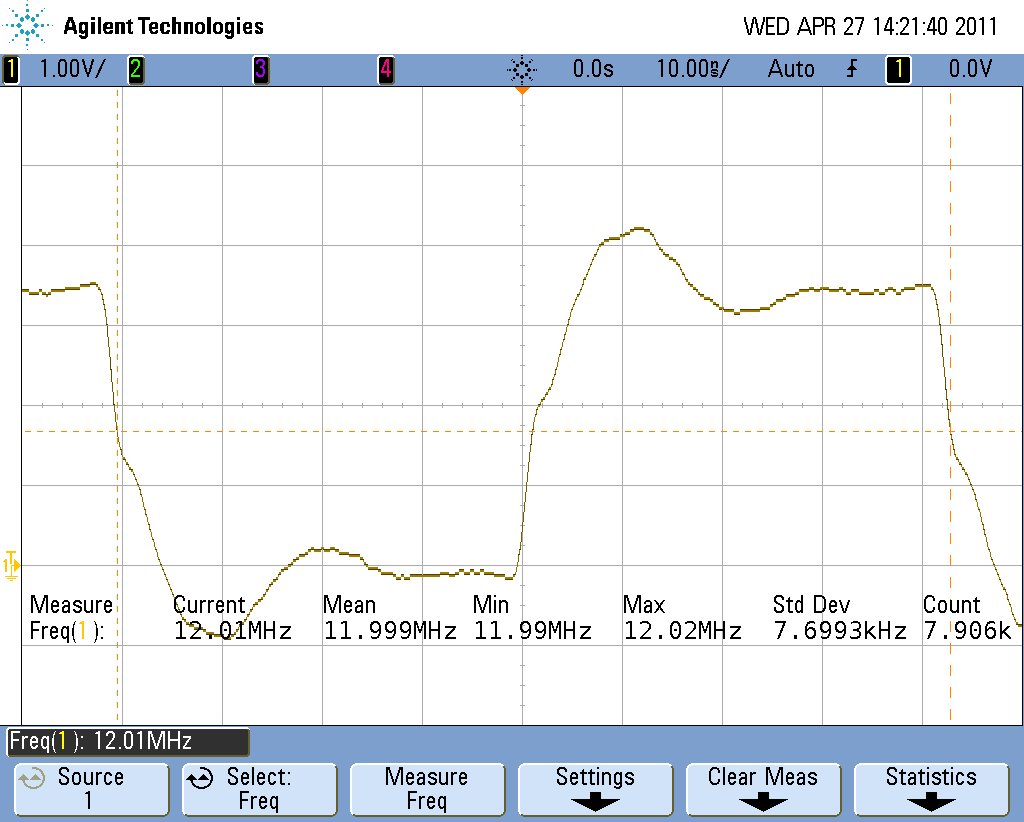
\includegraphics[width=\textwidth]{./img/codec_12M_clk.png}
	\caption{Output waveform of the clock generator}
	\label{fig:codec12Mclk}
\end{figure}

\subsubsection{Analogue}
The frequency response of the signal conditioning amplifier was tested, to check it would provide the correct reduction.
A sine wave at 5.03V peak to peak was applied at the input of one of the signal conditioners, and an oscilloscope probe connected to the output.
The frequency of the input sine wave was then changed and the output peak to peak voltage measured at each frequency.
This resulted in the graph shown by figure \ref{fig:sigcondtest}.

\begin{sidewaysfigure}
	\centering
	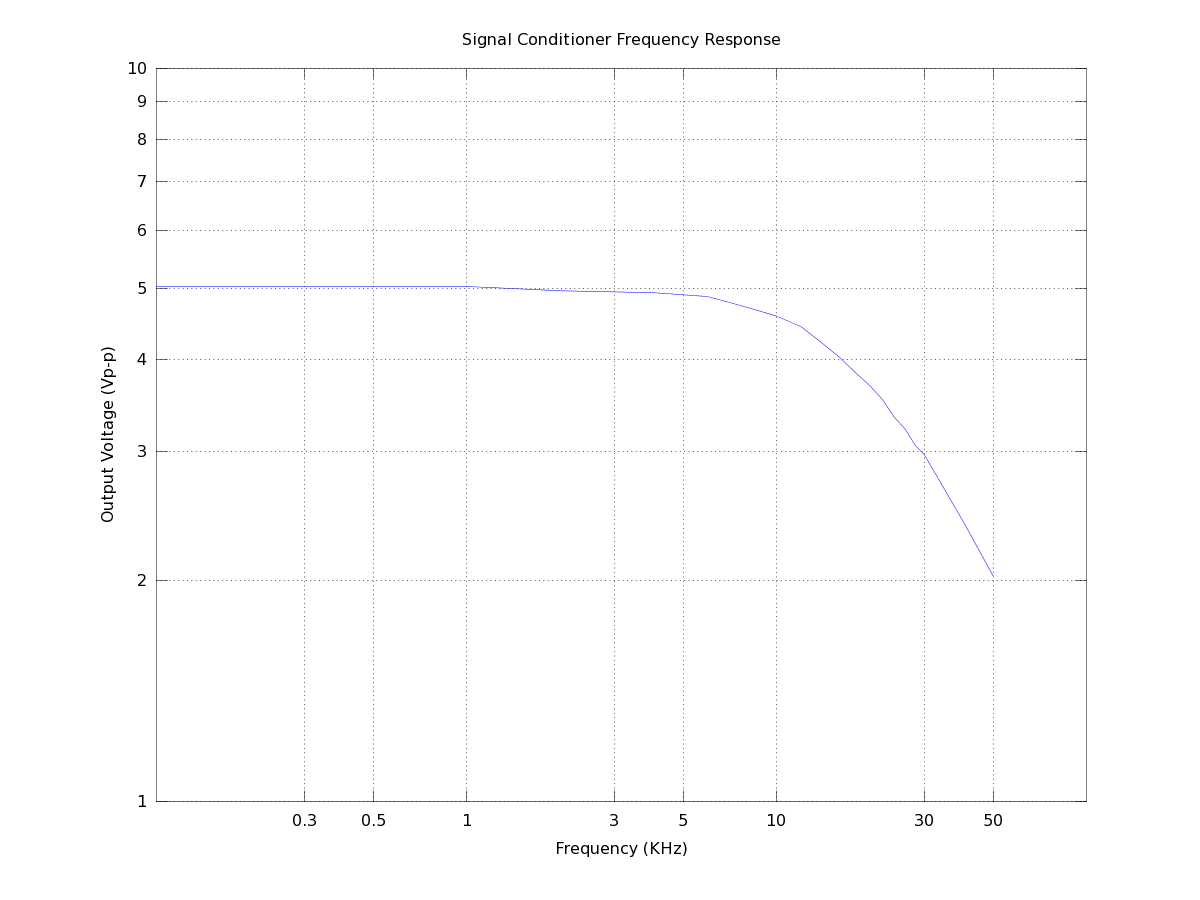
\includegraphics[width=\textwidth]{./img/sigcondtest.png}
	\caption{The frequency response of the signal conditioning amplifier}
	\label{fig:sigcondtest}
\end{sidewaysfigure}

\noindent This graph shows that the response of the amplifier matches the simulation (figure \ref{fig:sigcondmodel}).
Therefore the signal conditioning amplifier performs as expected.
